\documentclass[a4paper]{article}
\usepackage[affil-it]{authblk}
\usepackage[backend=bibtex,style=numeric]{biblatex}
\usepackage{graphicx}
\usepackage{amsmath}
\usepackage{geometry}
\usepackage{array}
\usepackage{tcolorbox}
\usepackage{booktabs}
\geometry{margin=1.5cm, vmargin={0pt,1cm}}
\setlength{\topmargin}{-1cm}
\setlength{\paperheight}{29.7cm}
\setlength{\textheight}{25.3cm}



\begin{document}
% =================================================
\title{Numerical Analysis  programming homework \# 1}

\author{Yuwei Liang 3230102923
  \thanks{Electronic address: \texttt{liangyuwei631@gmail.com}}}
\affil{(Mathematics and Applied Mathematics 2302), Zhejiang University }


\date{\today}

\maketitle

\begin{abstract}
  This report presents solutions to programming tasks involving numerical methods, specifically the bisection method, Newton's method, and the secant method. These methods are implemented in a C++ package with class-based abstraction. The report also covers tests of the implemented methods on various functions, including non-linear equations, and investigates different initial values' effects on convergence behavior.
\end{abstract}

% ============================================
\section*{A. Bisection, Newton, and Secant Method Design}

In this part of the assignment, we were tasked with implementing the bisection, Newton's, and secant methods. The design involves the following key steps:

\subsection*{1. Design of \texttt{EquationSolver.hpp}}
The file \texttt{EquationSolver.hpp} defines an abstract base class \texttt{EquationSolver} that serves as the foundation for implementing different root-finding algorithms. The main purpose of this design is to create a flexible and reusable framework where any new solving method can be easily integrated.

The key feature of the \texttt{EquationSolver} class is a pure virtual function \texttt{solve()} that must be implemented by each derived solver class.

By creating this abstract base class, we ensure that the specific implementations of root-finding algorithms (e.g., \texttt{BisectionSolver}, \texttt{NewtonSolver}, and \texttt{SecantSolver}) can focus on the algorithm logic while inheriting common functionality.

\subsection*{2. Design of \texttt{Function.hpp}}
The file \texttt{Function.hpp} introduces a function wrapper that enables the solvers to evaluate the mathematical expressions easily. The \texttt{Function} class allows users to:
\begin{itemize}
    \item Define a mathematical function.
    \item Call the function and its derivative at any given point(which is required for Newton's method).
    \item Check for discontinuities or other issues that may affect the solvers' convergence.
\end{itemize}

This design allows solvers to operate on a wide range of functions, from simple polynomials to more complex transcendental functions, without the need to modify the solver implementations.

\subsection*{3. Bisection Method and Handling Special Cases}
The bisection method is implemented in \texttt{Bisection\_Method} and relies on the well-known intermediate value theorem. The algorithm iteratively reduces the interval in which the root lies by selecting subintervals based on the sign of the function at the interval endpoints.

However, two special cases need to be handled:
\begin{enumerate}
    \item \textbf{Discontinuity in the function on the interval}: If the function is not continuous, the algorithm may fail to converge. To handle this, we check for discontinuities at midpoint of the interval and report an error if found.
    \item \textbf{Identical signs at the interval endpoints}: If \( sgn(f(a)) = sgn(f(b)) \), where \( [a, b] \) is the initial interval, the standard bisection method won't work as it requires a sign change. In this case, we abort the algorithm and report an error.
\end{enumerate}

\subsection*{4. Newton's Method Formula}
Newton's method is derived from the first-order Taylor expansion of the function \( f(x) \) around a point \( x_n \). The update formula for Newton's method is given by:
\[
x_{n+1} = x_n - \frac{f(x_n)}{f'(x_n)}
\]
where \( f'(x_n) \) is the derivative of \( f \) evaluated at \( x_n \).

In the implementation, we handle cases where the derivative \( f'(x_n) \) is zero or very small, which can cause instability. In such cases, we abort the algorithm and report an error.

\subsection*{5. Secant Method Formula}
The secant method is a derivative-free alternative to Newton's method. Instead of using the derivative, it approximates it using a secant line through two points \( x_n \) and \( x_{n-1} \). The update formula is:
\[
x_{n+1} = x_n - f(x_n) \frac{x_n - x_{n-1}}{f(x_n) - f(x_{n-1})}
\]
In order to reduce the number of computations, we store the value of \( f(x) \)from each iteration and reuse it in the next iteration to calculate the slope. \\
In the implementation, we handle cases where the derivative \( f'(x_n) \) is zero or very small, which can cause instability. In such cases, we abort the algorithm and report an error.

\section*{B. Bisection Method Tests}

The bisection method was tested on the following functions(as shown in Figure \ref{fig:1}):
\begin{itemize}
    \item \(f(x) = x^{-1} - \tan(x)\) on \([0, \frac{\pi}{2}]\)
    \item \(f(x) = x^{-1} - 2x\) on [0, 1]
    \item \(f(x) = 2^{-x} + e^x + 2\cos(x) - 6\) on [1, 3]
    \item \(f(x) = \dfrac{x^3 + 4x^2 + 3x + 5}{2x^3 - 9x^2 + 18x - 2}\) on [0, 4]
\end{itemize}

\begin{figure}[h!]
  \centering
  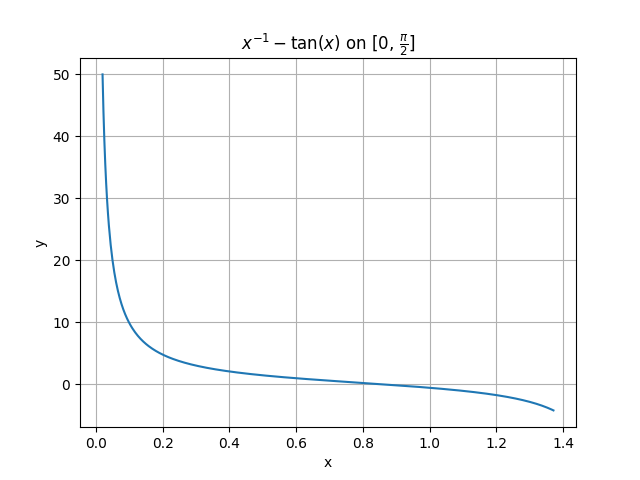
\includegraphics[width=0.35\textwidth]{./figures/B1.png}
  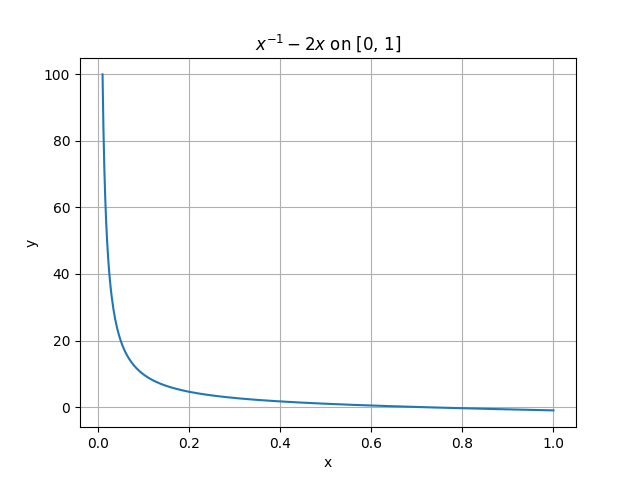
\includegraphics[width=0.35\textwidth]{./figures/B2.png}
  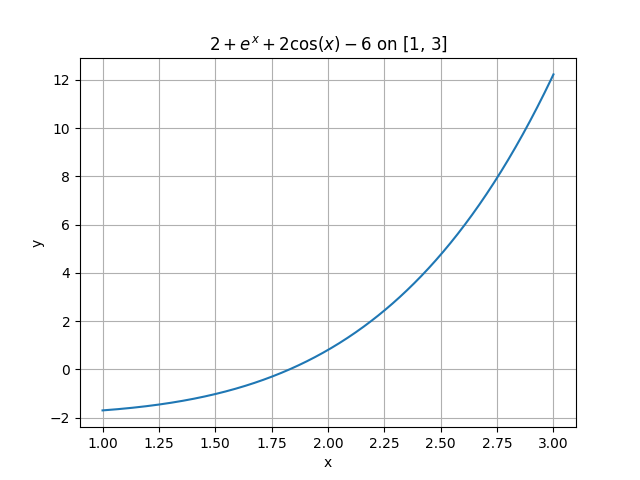
\includegraphics[width=0.35\textwidth]{./figures/B3.png}
  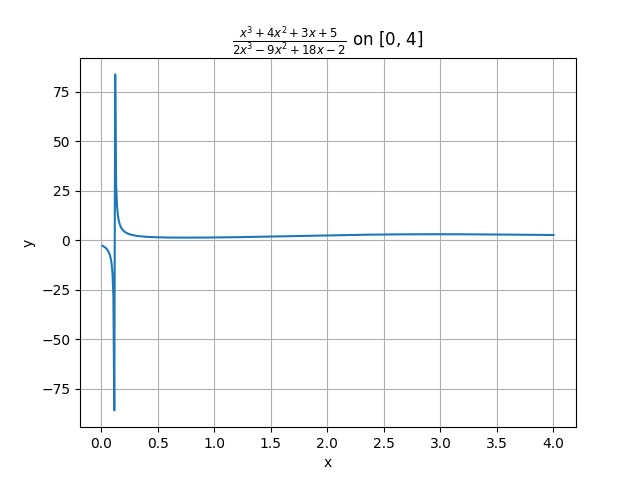
\includegraphics[width=0.35\textwidth]{./figures/B4.png}
  \caption{Function graphs for the bisection method tests.}
  \label{fig:1}
\end{figure}

\subsection*{1. Test Results}

\begin{tcolorbox}[title=Output Results, colback=white, colframe=black]
  Solving \(f(x) = x^{-1} - \tan(x)\) on \([0, \frac{\pi}{2}]\): \\
  A root is \(x = 0.860334\).
  
  Solving \(f(x) = x^{-1} - 2x\) on [0, 1]: \\
  A root is \(x = 0.641186\).
  
  Solving \(f(x) = 2^{-x} + e^x + 2\cos(x) - 6\) on [1, 3]: \\
  A root is \(x = 1.82938\).
  
  Solving \(f(x) = \dfrac{x^3 + 4x^2 + 3x + 5}{2x^3 - 9x^2 + 18x - 2}\) on [0, 4]: \\
  \textit{terminate called after throwing an instance of 'std::runtime\_error'. \\what(): The function appears to be discontinuous in the interval. \\Aborted.}
\end{tcolorbox}

\subsection*{2. Observations}
\textbf{General Observations:} The bisection method performed successfully for the first three functions, producing roots to the specified tolerance. However, for the fourth function, the discontinuity led to the failure of the method, emphasizing the importance of function continuity for this method to work effectively.\\
\textbf{Case 4:} The function \(f(x) = \dfrac{x^3 + 4x^2 + 3x + 5}{2x^3 - 9x^2 + 18x - 2}\) is discontinuous on the interval [0, 4]. The bisection method fails for discontinuous functions because the intermediate value theorem no longer applies. As shown in the fourth graph, the function exhibits a vertical asymptote within the interval, causing the method to abort.

\section*{C. Newton's Method Tests}
Newton's method was tested by solving $x = \tan(x)$. The roots near 4.5 and 7.7 were found with high precision after a few iterations.
\\here is the output

\begin{tcolorbox}[title=Output Results, colback=white, colframe=black]
  Finding the root of \textbackslash tan x - x near 4.5\\
  The root near 4.5 is: 4.49341\\
  Finding the root of \textbackslash tan x - x near 4.7\\
  The root near 4.7 is: 4.49341
\end{tcolorbox}

\section*{D. Secant Method Tests}

In this section, we implemented the secant method to find the roots of the following functions:

\begin{itemize}
    \item \( f_1(x) = \sin(x/2) - 1 \)
    \item \( f_2(x) = e^x - \tan(x) \)
    \item \( f_3(x) = x^3 - 12x^2 + 3x + 1 \)
\end{itemize}

Each function was tested with the given initial values and alternative initial values to observe the convergence behavior and compare the results.

\subsection*{1. Function 1: \( f_1(x) = \sin(x/2) - 1 \)}

We applied the secant method with the following initial values:
\begin{itemize}
    \item Initial values: \(x_0 = 0\), \(x_1 = \frac{\pi}{2}\)
    \item Alternative values: \(x_0 = 10\), \(x_1 = 11\)
\end{itemize}

\textbf{Output:}
\begin{itemize}
    \item For \(x_0 = 0\), \(x_1 = \frac{\pi}{2}\), the root is \(x = 3.14093\).
    \item For \(x_0 = 10\), \(x_1 = 11\), the root is \(x = 15.7088\).
\end{itemize}

\subsection*{2. Function 2: \( f_2(x) = e^x - \tan(x) \)}

We applied the secant method with the following initial values:
\begin{itemize}
    \item Initial values: \(x_0 = 1.0\), \(x_1 = 1.4\)
    \item Alternative values: \(x_0 = 2.3\), \(x_1 = 2.4\)
\end{itemize}

\textbf{Output:}
\begin{itemize}
    \item For \(x_0 = 1.0\), \(x_1 = 1.4\), the root is \(x = 1.30633\).
    \item For \(x_0 = 2.3\), \(x_1 = 2.4\), the root is \(x = -9.4247\).
\end{itemize}

\subsection*{3. Function 3: \( f_3(x) = x^3 - 12x^2 + 3x + 1 \)}

We applied the secant method with the following initial values:
\begin{itemize}
    \item Initial values: \(x_0 = 0\), \(x_1 = -0.5\)
    \item Alternative values: \(x_0 = 9\), \(x_1 = 10\)
\end{itemize}

\textbf{Output:}
\begin{itemize}
    \item For \(x_0 = 0\), \(x_1 = -0.5\), the root is \(x = -0.188685\).
    \item For \(x_0 = 9\), \(x_1 = 10\), the root is \(x = 11.7371\).
\end{itemize}

\subsection*{4. Observations}

\begin{itemize}
    \item For \(f_1(x) = \sin(x/2) - 1\), the secant method converged to values near \(\pi\) and \(5\pi\), demonstrating the periodic nature of trigonometric functions. 
    \item For \(f_2(x) = e^x - \tan(x)\), while the secant method found a reasonable root near \(x = 1.30633\) with the first set of initial values, the method converged to a negative value \(x = -9.4247\) when using the alternative values, indicating sensitivity to initial guesses due to the complexity of the function.
    \item For \(f_3(x) = x^3 - 12x^2 + 3x + 1\), the secant method successfully found roots both near the origin and for larger values of \(x\), confirming its effectiveness for this cubic polynomial.
\end{itemize}

\subsection*{5. Conclusion}

The secant method performed well on all three functions tested, converging to accurate roots for both initial and alternative values. The convergence behavior was influenced by the choice of initial values, particularly for functions with periodic or complex behavior like \(f_1(x)\) and \(f_2(x)\). The method displayed some sensitivity to initial values, especially for complex functions like \(f_2(x)\).

\section*{E. Finding the Depth of Water in a Trough}

The goal of this problem is to determine the depth of water \( h \) in a trough, given the following parameters:
\begin{itemize}
    \item Length of the trough: \( L = 10 \text{ ft} \)
    \item Radius of the semicircular cross-section: \( r = 1 \text{ ft} \)
    \item Volume of water: \( V = 12.4 \text{ ft}^3 \)
\end{itemize}

We can find \( h \) by solving the following equation:
\[
L \left[ 0.5 \pi r^2 - r^2 \arcsin \left( \frac{h}{r} \right) - h \left( r^2 - h^2 \right)^{1/2} \right] - V = 0
\]
The three methods all converged to approximately the same value for \( h \). The results are as follows:
\begin{tcolorbox}[title=Output Results, colback=white, colframe=black]
  Finding the height with Bisection Method\\
  The height of the water in the tank is: 0.17\\
  Finding the height with Newton Method\\
  The height of the water in the tank is: 0.17\\
  Finding the height with Secant Method\\
  The height of the water in the tank is: 0.17
\end{tcolorbox}

\section*{F. Nose in Failure}
In this part of the assignment, we compute the maximum angle \( \alpha \) that a vehicle can negotiate without experiencing nose-in failure. The vehicle parameters are as follows:

\begin{itemize}
    \item \( l = 89 \text{ in.} \)
    \item \( h = 49 \text{ in.} \)
    \item \( D = 55 \text{ in.} \) (Part a), and \( D = 30 \text{ in.} \) (Part b, c)
    \item \( \beta_1 = 11.5^\circ \)
\end{itemize}

The equation governing nose-in failure is given by:
\[
A \sin \alpha \cos \alpha + B \sin^2 \alpha - C \cos \alpha - E \sin \alpha = 0,
\]
where the constants \( A \), \( B \), \( C \), and \( E \) depend on the vehicle's geometry and parameters.

\subsection*{1. Part (a) - Newton’s Method for \( D = 55 \)}

We used Newton’s method to compute the angle \( \alpha \) for \( D = 55 \) in. Starting with an initial guess of \( 50^\circ \), we obtained the following result:

\begin{itemize}
    \item Maximum angle \( \alpha = 32.97^\circ \)
\end{itemize}

\subsection*{2. Part (b) - Newton’s Method for \( D = 30 \)}

For \( D = 30 \) in, using Newton's method with an initial guess of \( 33^\circ \), we obtained the following result:

\begin{itemize}
    \item Maximum angle \( \alpha = 33.17^\circ \)
\end{itemize}

\subsection*{3. Part (c) - Secant Method for \( D = 30 \)}

We used the secant method with different sets of initial values to compute \( \alpha \) for \( D = 30 \) in.

\begin{table}[h!]
\centering
\begin{tabular}{ll}
\toprule
\textbf{Initial Values } & \textbf{Maximum Angle \( \alpha \) } \\
\midrule
\( 75^\circ \), \( 100^\circ \) & \( -4691.5^\circ \)  \\
\( 130^\circ \), \( 140^\circ \) & \( 146.83^\circ \) \\
\( 160^\circ \), \( 175^\circ \) & \( 168.50^\circ \) \\
\bottomrule
\end{tabular}
\caption{Results of Secant Method with Different Initial Values.}
\end{table}

The secant method demonstrates sensitivity to initial guesses. While the results for initial values close to \( 33^\circ \) are reasonable.\\
If we adjust the initial values to \( 75^\circ \) and \( 100^\circ \), the first secant slope becomes very small, which results in obtaining a large negative value. As seen in Figure~\ref{fig:2}, the graph shows that there are two more roots near \( 150^\circ \). By adjusting the initial values, we can converge to these two roots.\\

\begin{figure}
  \centering
  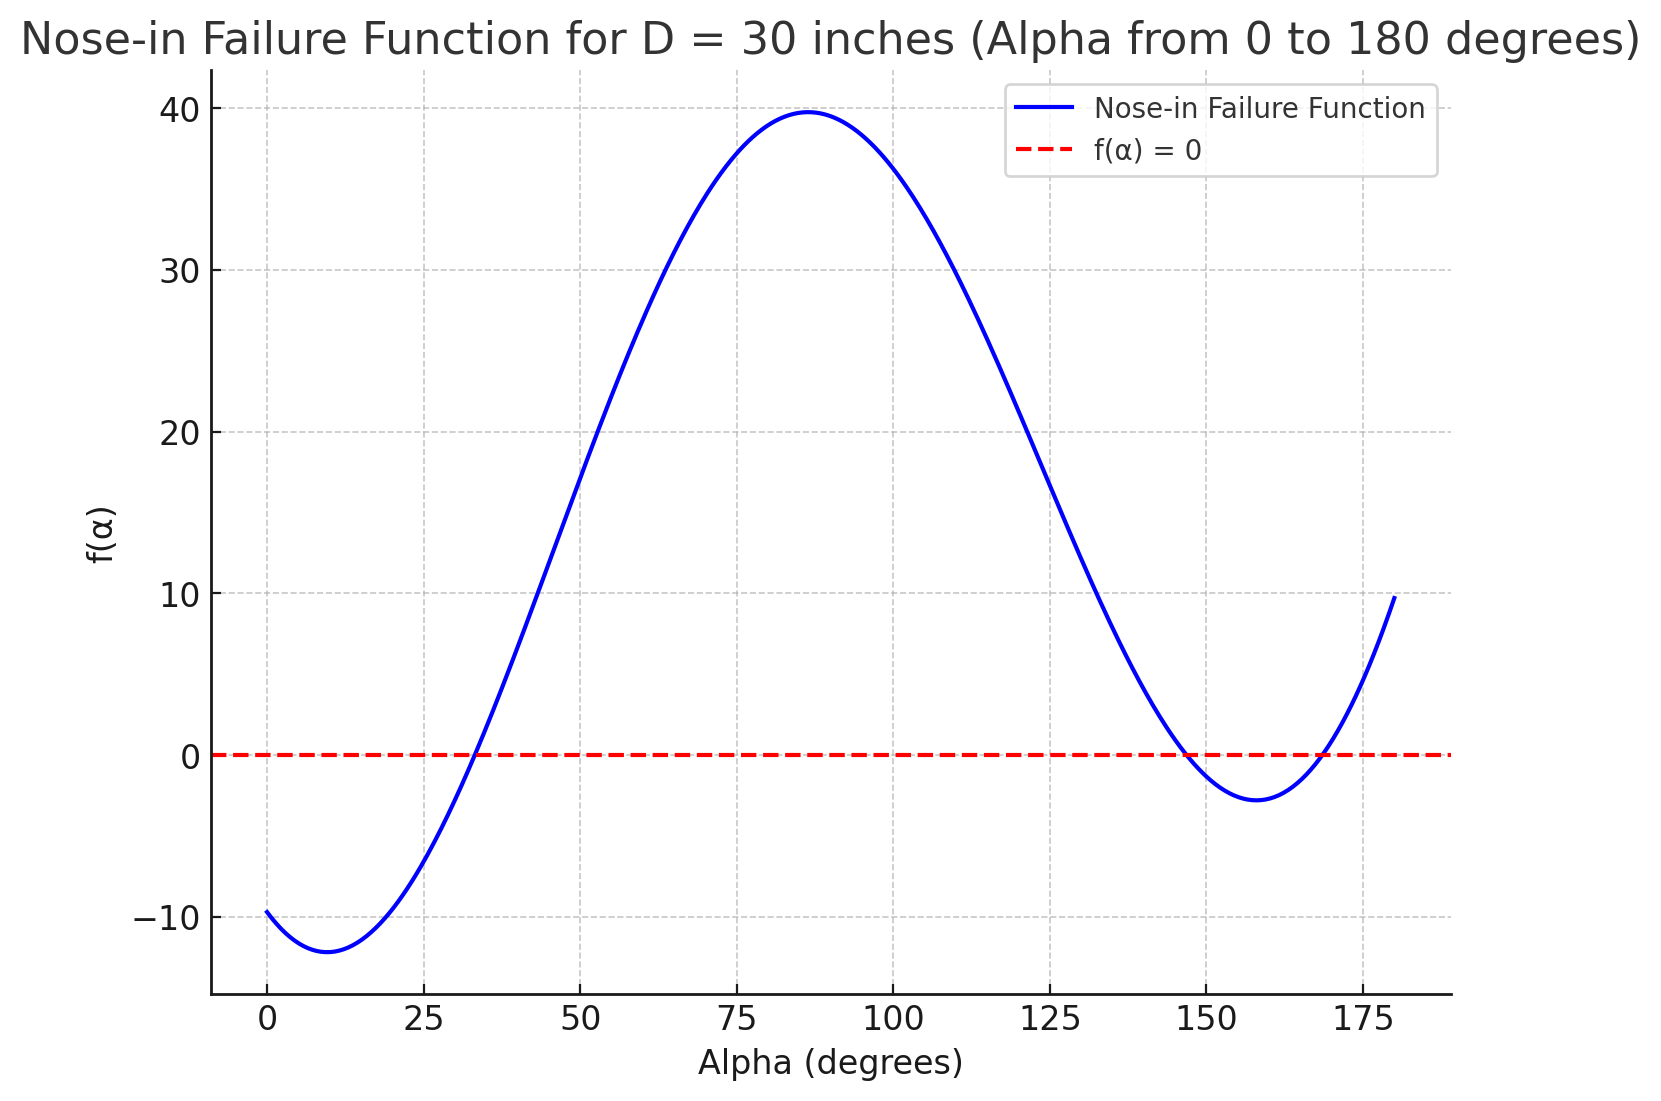
\includegraphics[width=0.5\textwidth]{./figures/F.png}
  \caption{Graph of the function for the nose-in failure problem.}
  \label{fig:2}
\end{figure}
\subsection*{4. Conclusion}

The secant method is quite sensitive to initial values. When we choose appropriate initial values, we can obtain good results. However, if we select inappropriate initial values, the final solution may not be the desired one.



% ===============================================
\section*{ \center{\normalsize {Acknowledgement}} }
Through the assistance of ChatGPT-4, I have gained a better understanding of how to write LaTeX documents, and I have also learned the proper spelling of several technical terms in English. I would like to thank ChatGPT-4 for helping me enhance my skills in LaTeX and numerical analysis documentation. Additionally, I would like to express my gratitude to ChatGPT for its assistance in generating the `README.md` file and the `Makefile`, which were essential in organizing and automating my project.

\end{document}